\documentclass[a4paper,fleqn]{cas-sc}

\usepackage[numbers,sort&compress]{natbib}
\usepackage{amsmath,amssymb}
\usepackage{booktabs}
\usepackage{graphicx}
\usepackage{microtype}
\usepackage{siunitx}
\usepackage{tabularx}
\usepackage{xcolor}
\usepackage{tikz}
\usetikzlibrary{arrows.meta,positioning,fit,shapes.geometric}

\definecolor{FaceBlue}{HTML}{0072B2}
\definecolor{SideOrange}{HTML}{E69F00}
\definecolor{FuseGreen}{HTML}{009E73}
\definecolor{EvalGray}{HTML}{666666}
\definecolor{PendingRed}{HTML}{A51C30}
\newcommand{\resultpending}[1]{\textcolor{PendingRed}{\textbf{[Pending: #1]}}}
\newcommand{\pendingcell}{\textcolor{PendingRed}{\textbf{Pending}}}
\newcommand{\submissionpending}[1]{\textcolor{PendingRed}{\textbf{[Submission item: #1]}}}
\newcommand{\methodname}{Rotation-Aware Self-Supervised Fusion}

\begin{document}
\let\WriteBookmarks\relax
\def\floatpagepagefraction{1}
\def\textpagefraction{.001}

\shorttitle{Rotation-Aware Two-View 3D Pose Fusion}
\shortauthors{K. Chen}

\title[mode=title]{Rotation-Aware Self-Supervised Fusion of Temporally Aligned Two-View 3D Human Poses}

\author[1]{Kaixu Chen}
\cormark[1]
\ead{chenkaixusan@gmail.com}
\credit{Conceptualization, Methodology, Software, Validation, Formal analysis, Investigation, Data curation, Visualization, Writing -- original draft, Writing -- review and editing}
\affiliation[1]{organization={CCS}}
\cortext[1]{Corresponding author}

\begin{abstract}
Monocular three-dimensional pose estimates from different views retain
view-dependent coordinate, depth, and occlusion errors. We study
post-estimation fusion of two temporally aligned 3D keypoint streams without
camera parameters or 3D reference poses during training. The proposed A6
framework canonicalizes both streams and applies a view-swap-invariant temporal
network that predicts a bounded residual over a quality-weighted mean.
Reproducible corruptions, cross-view consensus, skeletal structure, temporal
dynamics, and complete-cycle rotation provide self-supervision. On 137 people,
body-frame averaging reduced mean distance to a same-video triangulated
pseudo-reference by 47.54\% relative to world-coordinate averaging. On the
held-out test set ($N=14$), A6 obtained 60.78~mm after sequence-level
similarity alignment; it was statistically indistinguishable from arithmetic
averaging (60.85~mm) and A5 (60.80~mm). A6 is therefore retained as the complete
constrained objective, not as a positional-accuracy winner. Limited external
testing against Unity native 3D (199 samples, one avatar/environment) found no
zero-shot improvement for A6 over direct 3D averaging (178.506 versus
166.537~mm); calibrated 2D triangulation was substantially better
(30.259~mm), but represents a different input regime. Person-disjoint
out-of-fold A6 inference additionally yielded 928 cycles from 80
elderly-labeled and 57 student-labeled participants. Centered mixed models found
cohort differences in angular speed and log dimensionless jerk, but
source-matched sensitivity showed materially smaller or absent effects in other
pose streams. These observational, model-derived descriptors are not causal
ageing or clinical findings.
\end{abstract}

\begin{highlights}
\item Fusion uses two monocular 3D pose streams without camera parameters.
\item Pelvis-thorax rotations guide a swap-invariant residual temporal model.
\item Self-supervision combines recovery, structure, motion, and cycle losses.
\item Evaluation separates held-out, descriptive, and Unity evidence populations.
\item Person-disjoint A6 outputs support cohort and repeated-cycle analysis.
\end{highlights}

\begin{keywords}
3D human pose \sep multi-view fusion \sep self-supervised learning \sep
temporal convolution \sep trunk rotation \sep markerless motion analysis
\end{keywords}

\maketitle

\section{Introduction}
\label{sec:introduction}

Three-dimensional human pose estimation from ordinary video has become an
accessible alternative to specialized motion-capture laboratories. Modern
single-image systems can recover a dense articulated body representation under
varied appearance and imaging conditions; SAM 3D Body, for example, predicts a
full-body mesh based on the Momentum Human Rig representation
\citep{Yang2026SAM3DBody}. Nevertheless, a monocular 3D reconstruction remains
view dependent. Depth ambiguity, self-occlusion, motion blur, truncation, and
imperfect scale recovery affect frontal and lateral observations differently.
When two cameras observe the same movement, their predictions therefore contain
both complementary information and incompatible errors.

Most multi-view 3D pose research resolves this problem before or during 3D
estimation. Calibrated approaches combine image features or 2D heatmaps and
triangulate a common 3D pose \citep{Iskakov2019Learnable,Qiu2019CrossView,
Remelli2020Lightweight}. More recent methods relax calibration or 3D-label
requirements, but they still begin from images or 2D observations and jointly
infer cameras, 2D poses, or 3D locations
\citep{Kim2022CrossViewSelfFusion,Usman2022MetaPose,Jiang2023Probabilistic,
Srivastav2024SelfPose3D}. These formulations do not directly address a common
downstream situation: two complete monocular 3D pose streams already exist, the
camera geometry is unavailable or unreliable, and the desired output is a
single temporally coherent 3D sequence.

Naive averaging is inadequate in this setting. The two streams may use
different translations, orientations, and scales, and a method that minimizes
coordinate noise can suppress the rapid trunk rotation that is central to the
movement under study. This distinction matters for gymnastics and other
rotation-dominant actions, where a visually smooth sequence is not necessarily
a faithful sequence. A useful fusion method must therefore reduce view-specific
artifacts while preserving angular range and peak motion.

This paper formulates \emph{post-estimation two-view 3D pose fusion}. The method
receives temporally aligned face-view and side-view 3D keypoints and produces a
full fused sequence without camera parameters, manually labeled 3D poses, or a
triangulated target during training. Each view is canonicalized in a
pelvis-centered, trial-scaled body frame. Pelvis-to-thorax relative rotations,
wrapped axial angle, angular derivatives, per-view reliability, and symmetric
cross-view disagreement are then supplied to a view-swap-invariant temporal
network. The network predicts a bounded correction to a deterministic
quality-weighted mean. Training uses seeded synthetic corruptions together with
consensus, skeletal, temporal, and complete-cycle rotation constraints.

The study is motivated by the following research question: \emph{Can two
temporally aligned monocular 3D pose streams be fused without camera calibration
or 3D supervision so that cross-view artifacts decrease without attenuating the
trunk-rotation dynamics of a complete movement cycle?} We evaluate two distinct
properties rather than collapsing them into one claim. First, agreement with a
triangulated stream is reported as agreement with a shared upstream
pseudo-reference. Second, reference-independent diagnostics quantify corruption
recovery, skeletal consistency, view-swap invariance, temporal smoothness, and
rotation preservation. Because no independent motion-capture measurements are
available, the study does not claim absolute positional or biomechanical
accuracy. A limited synthetic benchmark against Unity native 3D separately
tests transfer outside the private videos and exposes the boundary between
uncalibrated direct-3D fusion and calibrated 2D triangulation.

A secondary application question asks whether person-disjoint A6 outputs can
support two complementary comparisons: differences between the
elderly-labeled and student-labeled participant groups, and differences among
repeated cycles within the same person. This analysis is observational. The
cohort labels do not identify causal ageing effects, and the fused descriptors
are not clinical measurements.

The contributions are as follows:
\begin{itemize}
  \item We define a practical post-estimation fusion problem in which two
  monocular 3D pose streams, rather than images or 2D heatmaps, are the inputs.
  \item We introduce a rotation-aware, view-swap-invariant residual temporal
  model that combines canonical 3D coordinates with explicit pelvis--thorax
  rotation and deterministic quality features.
  \item We construct a self-supervised objective from reproducible corruptions,
  reliable cross-view consensus, skeletal structure, adaptive temporal dynamics,
  and complete-cycle axial range, while isolating triangulated poses from model
  training and checkpoint selection.
  \item We provide an auditable evaluation protocol that keeps the deterministic
  results, the 14-person held-out learned comparison, descriptive all-person
  diagnostics, and Unity native-3D evidence separate.
  \item We demonstrate a downstream person-disjoint analysis that separates
  adjusted cohort contrasts, within-person cycle variability, and repetition
  trends, with pose-source and limited seed sensitivity checks.
\end{itemize}

The primary learned comparison uses the frozen 14-person test split; the
96-person training and 27-person validation sets are not reused for its
generalization claim. Inference over all 137 people is descriptive only.
Downstream A6 analysis uses ten person-disjoint outer folds and is qualified by
the same centered mixed-model estimand applied to single-view and deterministic
pose sources. These boundaries keep pseudo-reference agreement, limited
synthetic external validity, motion preservation, and observational group
comparisons distinct.

\section{Related work}
\label{sec:related}

\subsection{Monocular and temporal 3D pose estimation}

Monocular 3D pose estimation must resolve depth from incomplete visual
evidence. Temporal models reduce framewise ambiguity by exploiting motion
context. VideoPose3D demonstrated that dilated temporal convolutions can model
long sequences of 2D keypoints efficiently, including in a semi-supervised
setting \citep{Pavllo2019VideoPose3D}. Temporal attention and multi-scale
dilations have likewise been used to reduce jitter and exploit longer context
\citep{Liu2020TemporalAttention}. Our method also uses dilated temporal
convolutions, but it does not lift a 2D sequence. It receives two existing 3D
streams and learns how to combine their complementary reliability.

SAM 3D Body provides the upstream representation in this study
\citep{Yang2026SAM3DBody}. Its MHR output includes body, hand, and foot joints,
giving a 70-joint sequence after inference. We treat this estimator as fixed.
Consequently, the proposed contribution is neither a new body model nor a new
image-to-pose network; it is a downstream fusion layer whose failure modes and
claims must remain conditional on the upstream estimator.

\subsection{Calibrated multi-view fusion and triangulation}

Classical multi-view pose pipelines recover 3D points from synchronized 2D
correspondences and camera projection matrices. Learnable triangulation adds
confidence weighting or volumetric aggregation to this geometry
\citep{Iskakov2019Learnable}. Cross-view fusion can also be introduced at the
image-feature or 2D-pose stage before a structured 3D recovery step
\citep{Qiu2019CrossView}. Camera-disentangled representations reduce the cost of
volumetric processing while retaining calibrated geometric lifting
\citep{Remelli2020Lightweight}. Generalizable triangulation addresses changes in
camera arrangement \citep{Bartol2022Generalizable}, and probabilistic
triangulation models uncertain camera pose for nominally uncalibrated scenes
\citep{Jiang2023Probabilistic}.

These methods estimate 3D structure from multi-view image evidence. By contrast,
our inputs are already 3D, and the method neither receives projection matrices
nor reprojects to images. The two problem classes are complementary. In this
study, conventional triangulation is retained only as an evaluation
pseudo-reference, not as a target used by the fusion learner.

\subsection{Self-supervised multi-view learning}

Multi-view consistency is a strong source of supervision when 3D labels are
scarce. Cross-View Self-Fusion refines 2D observations across uncalibrated views
and trains a monocular lifting network; only one view is needed at inference
\citep{Kim2022CrossViewSelfFusion}. MetaPose jointly estimates camera and pose
from multiple 2D keypoint sets without 3D supervision
\citep{Usman2022MetaPose}. SelfPose3D uses calibrated multi-view images and 2D
pseudo-poses to learn multi-person 3D localization and pose without manual 2D or
3D labels \citep{Srivastav2024SelfPose3D}.

Our use of ``self-supervised fusion'' is therefore narrower. Two views remain
required at inference, and the output is the final fused 3D keypoint sequence.
No camera is estimated. The supervision comes from controlled perturbation of
the observed 3D streams, high-confidence agreement between them, and explicit
sequence structure. This avoids training on the triangulated evaluation stream,
but it does not make the two monocular inputs statistically independent.

\subsection{Rotation representation and applied motion analysis}

Rotation-aware processing requires care because common low-dimensional rotation
parameterizations contain discontinuities. Continuous neural rotation
representations have been studied explicitly \citep{Zhou2019Rotation}. Rather
than regress an unconstrained rotation parameterization, our network predicts
bounded keypoint residuals and derives a proper $\mathrm{SO}(3)$
pelvis--thorax rotation from the resulting skeleton. Circular differences are
used for the signed axial angle so that the $-\pi/\pi$ boundary does not create a
spurious error.

Applied markerless systems such as OpenCap use calibrated smartphone video,
triangulated 2D keypoints, a Mocap-trained marker model, musculoskeletal
constraints, and laboratory validation \citep{Uhlrich2023OpenCap}. That pipeline
supports biomechanical outputs that are outside the scope of this work. We
study uncalibrated pose-stream fusion and return 3D keypoints only. The method is
intended for robust motion representation and comparative analysis, not for
clinical kinetics or validated joint moments.

\begin{table*}[t]
\centering
\caption{Methodological positioning. ``Two 3D streams'' means that complete
per-view 3D poses, rather than images or 2D keypoints, are the fusion inputs.}
\label{tab:positioning}
\scriptsize
\setlength{\tabcolsep}{3pt}
\begin{tabularx}{\linewidth}{p{0.18\linewidth} p{0.15\linewidth}
  >{\centering\arraybackslash}p{0.11\linewidth}
  >{\centering\arraybackslash}p{0.11\linewidth}
  >{\centering\arraybackslash}p{0.11\linewidth} X}
\toprule
Method family & Fusion input & \makecell{Camera\\parameters} &
\makecell{3D labels\\for training} & \makecell{Two views\\at inference} & Primary output \\
\midrule
Learnable triangulation \citep{Iskakov2019Learnable} & Images/2D heatmaps & Required & Commonly used & Yes & Geometric 3D pose \\
Uncalibrated triangulation \citep{Jiang2023Probabilistic} & Images/2D features & Estimated distribution & Used by embedded estimator & Yes & Camera-aware 3D pose \\
Cross-View Self-Fusion \citep{Kim2022CrossViewSelfFusion} & Multi-view 2D poses & Not required & No & No & Trained monocular estimator \\
MetaPose \citep{Usman2022MetaPose} & Multi-view 2D keypoints & Estimated & No & Yes & Camera and 3D pose \\
SelfPose3D \citep{Srivastav2024SelfPose3D} & Calibrated images and 2D pseudo-poses & Required & No manual labels & Yes & Multi-person 3D pose \\
Proposed method & Two 3D streams & Not used & No & Yes & Fused temporal 3D pose \\
\bottomrule
\end{tabularx}
\end{table*}


Table~\ref{tab:positioning} summarizes the resulting methodological boundary.
The closest prior work shares multi-view self-supervision, but differs in input
space, inference-time view count, and output objective. The novel claim is thus
the combination of post-estimation 3D fusion, explicit rotation preservation,
and label-free temporal training, not any single component such as a temporal
convolution, canonical frame, or skeletal loss.

\section{Problem formulation}
\label{sec:problem}

\subsection{Inputs and temporal correspondence}

For a movement trial, let
\begin{equation}
  \mathbf{X}^{f},\mathbf{X}^{s}\in\mathbb{R}^{T\times J\times 3}
\end{equation}
denote the face-view and side-view monocular 3D keypoints after temporal
alignment, where $T$ is the number of overlapping frames and $J=70$ is the MHR
joint count. Binary masks
$\mathbf{M}^{f},\mathbf{M}^{s}\in\{0,1\}^{T\times J}$ identify finite, observed
keypoints. Frame time is represented by timestamps $\tau_t$ and physical
intervals $\Delta t_t=\tau_t-\tau_{t-1}$.

The two camera streams are not assumed to begin simultaneously. An upstream
cycle-segmentation stage estimates a side-to-face frame offset
$o_{s\rightarrow f}$ and stores both the offset and the face/side frame ranges
of every cycle. The fusion loader uses this stored offset exactly. It constructs
the overlapping frame maps and then intersects both maps with the recorded cycle
bounds. It does not estimate a second dynamic-time-warping offset and does not
fall back to a different synchronization rule. Therefore, timing is an explicit
input contract rather than a latent correction expected from the network.

\subsection{Desired output}

The fusion function
\begin{equation}
  \widehat{\mathbf{X}} =
  F_{\phi}(\mathbf{X}^{f},\mathbf{M}^{f},
           \mathbf{X}^{s},\mathbf{M}^{s},\boldsymbol{\tau})
\end{equation}
returns one $T\times J\times3$ sequence and a validity mask. The final export is
expressed in a face-reference coordinate frame for compatibility with the
existing analysis pipeline. ``Face reference'' means that the fused canonical
pose is restored with the face stream's per-frame origin, orientation, and trial
scale. It is not a calibrated world coordinate system.

We impose four design requirements. First, fusion should be invariant to
interchanging the semantic input order:
\begin{equation}
 F_{\phi}(\mathbf{X}^{f},\mathbf{X}^{s})
 \approx F_{\phi}(\mathbf{X}^{s},\mathbf{X}^{f}).
 \label{eq:swap}
\end{equation}
Second, if one joint is valid in only one view, the valid observation should pass
through rather than be averaged with a missing value. Third, learned corrections
should be bounded so a weak pseudo-target cannot move the output arbitrarily far
from the observations. Fourth, fusion should preserve the signed pelvis--thorax
rotation, its range over a complete cycle, and rapid but plausible angular
changes.

\subsection{Supervision boundary}

Training may use only the two aligned SAM3D streams, their masks and timestamps,
the split-cycle metadata, and deterministic transformations or corruptions
derived from those variables. It may not read triangulated 3D poses, an
evaluation MPJPE, or any label derived from the triangulation output. Validation
and checkpoint selection use self-supervised measures only. The triangulated
stream is opened by a separate evaluation adapter after inference.

This boundary prevents direct target leakage but does not convert the
triangulated sequence into independent truth: it is produced from 2D keypoints
extracted from the same two videos. Accordingly, we call its distance measure
\emph{pseudo-reference agreement}. Absolute 3D accuracy would require an
independent reference such as synchronized marker-based motion capture or an
external benchmark with appropriate ground truth.

\begin{figure}
\centering
\resizebox{\linewidth}{!}{%
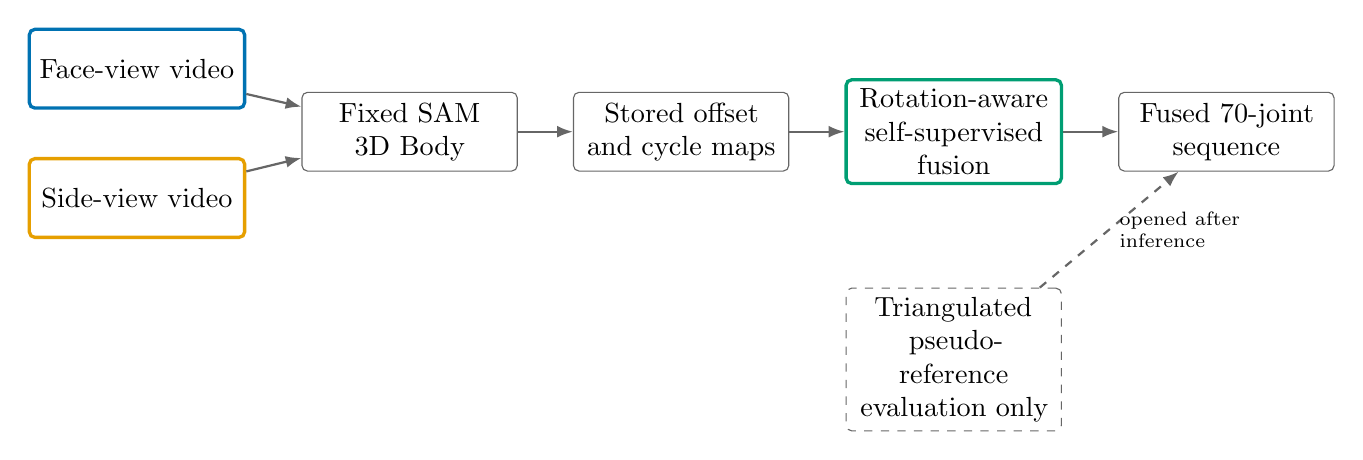
\begin{tikzpicture}[
  node distance=6mm and 7mm,
  box/.style={draw=EvalGray, rounded corners=2pt, align=center, minimum height=10mm, text width=25mm, fill=white},
  face/.style={box, draw=FaceBlue, very thick},
  side/.style={box, draw=SideOrange, very thick},
  fuse/.style={box, draw=FuseGreen, very thick},
  eval/.style={box, draw=EvalGray, dashed},
  arrow/.style={-{Latex[length=2mm]}, thick, draw=EvalGray}
]
\node[face] (facevideo) {Face-view video};
\node[side, below=of facevideo] (sidevideo) {Side-view video};
\node[box, right=of facevideo, yshift=-8mm] (sam) {Fixed SAM 3D Body};
\node[box, right=of sam] (split) {Stored offset and cycle maps};
\node[fuse, right=of split] (method) {Rotation-aware self-supervised fusion};
\node[box, right=of method] (output) {Fused 70-joint sequence};
\node[eval, below=13mm of method] (triangulation) {Triangulated pseudo-reference\\evaluation only};

\draw[arrow] (facevideo) -- (sam);
\draw[arrow] (sidevideo) -- (sam);
\draw[arrow] (sam) -- (split);
\draw[arrow] (split) -- (method);
\draw[arrow] (method) -- (output);
\draw[arrow, dashed] (triangulation) -- node[right, font=\scriptsize, align=left] {opened after\\inference} (output);
\end{tikzpicture}
}
\caption{Study boundary. The learned fusion path consumes only two monocular 3D
pose streams and split-cycle timing metadata. The triangulated stream is isolated
from training and checkpoint selection.}
\label{fig:pipeline}
\end{figure}


\section{Rotation-aware self-supervised fusion}
\label{sec:method}

\subsection{Method overview}

The method separates deterministic geometry from learned correction. Each
complete trial is first canonicalized independently for the face and side
streams. From the canonical poses we compute per-view pose, trunk-rotation, and
quality features together with symmetric cross-view disagreement. A fixed
quality-weighted fusion provides a conservative base pose. A shared view
encoder and a non-causal temporal convolutional network then predict a bounded
per-joint residual. Figure~\ref{fig:architecture} shows this data flow.

\begin{figure}
\centering
\resizebox{\linewidth}{!}{%
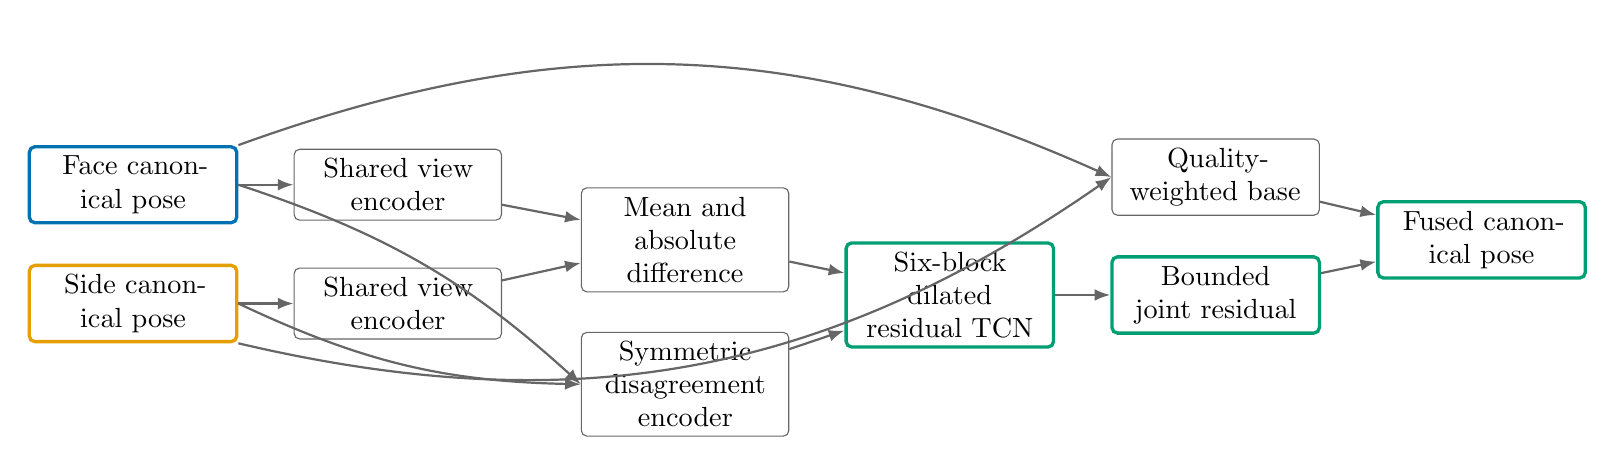
\begin{tikzpicture}[
  node distance=5mm and 7mm,
  box/.style={draw=EvalGray, rounded corners=2pt, align=center, minimum height=9mm, text width=24mm, fill=white},
  face/.style={box, draw=FaceBlue, very thick},
  side/.style={box, draw=SideOrange, very thick},
  fuse/.style={box, draw=FuseGreen, very thick},
  arrow/.style={-{Latex[length=2mm]}, thick, draw=EvalGray},
  note/.style={font=\scriptsize, align=center}
]
\node[face] (face) {Face canonical pose};
\node[side, below=of face] (side) {Side canonical pose};
\node[box, right=of face] (sharedf) {Shared view encoder};
\node[box, right=of side] (shareds) {Shared view encoder};
\node[box, right=10mm of sharedf, yshift=-7mm] (sym) {Mean and absolute difference};
\node[box, below=of sym] (cross) {Symmetric disagreement encoder};
\node[fuse, right=of sym, yshift=-7mm] (tcn) {Six-block dilated residual TCN};
\node[fuse, right=of tcn] (delta) {Bounded joint residual};
\node[box, above=of delta] (base) {Quality-weighted base};
\node[fuse, right=of delta, yshift=7mm] (out) {Fused canonical pose};

\draw[arrow] (face) -- (sharedf);
\draw[arrow] (side) -- (shareds);
\draw[arrow] (sharedf) -- (sym);
\draw[arrow] (shareds) -- (sym);
\draw[arrow] (face.east) to[bend left=12] (cross.west);
\draw[arrow] (side.east) to[bend right=12] (cross.west);
\draw[arrow] (sym) -- (tcn);
\draw[arrow] (cross) -- (tcn);
\draw[arrow] (tcn) -- (delta);
\draw[arrow] (face.north east) to[bend left=22] (base.west);
\draw[arrow] (side.south east) to[bend right=24] (base.west);
\draw[arrow] (base) -- (out);
\draw[arrow] (delta) -- (out);
\end{tikzpicture}
}
\caption{Fusion architecture. Both semantic views pass through one shared
encoder. Only symmetric combinations enter the residual TCN. The learned output
is a bounded correction to a detached quality-weighted base.}
\label{fig:architecture}
\end{figure}


\subsection{Pelvis-centered canonicalization}

For each view $v\in\{f,s\}$ and frame $t$, the pelvis origin
$\mathbf{o}^{v}_{t}$ is obtained from the configured pelvis joint or midpoint.
The lateral axis is the normalized right-to-left hip direction. The initial
vertical direction points from pelvis to thorax and is orthogonalized against
the lateral axis. Their cross product gives the third axis, after which the
lateral axis is reconstructed to ensure a right-handed orthonormal frame. We
write the resulting local-to-view rotation as
\begin{equation}
  \mathbf{R}^{v}_{p,t}=
  [\mathbf{e}^{v}_{x,t},\mathbf{e}^{v}_{y,t},\mathbf{e}^{v}_{z,t}]
  \in\mathrm{SO}(3).
\end{equation}
Degenerate frames retain the most recent observable transform for continuity,
while their frame-valid flag remains false so they cannot silently create
supervision.

A robust trial scale is defined independently in each stream as the median
valid pelvis--thorax distance,
\begin{equation}
  a^v=\operatorname{median}_{t\in\mathcal{V}^{v}}
  \lVert\mathbf{x}^{v}_{t,\mathrm{thorax}}-
  \mathbf{x}^{v}_{t,\mathrm{pelvis}}\rVert_2.
\end{equation}
Canonical keypoints are
\begin{equation}
  \widetilde{\mathbf{x}}^{v}_{t,j}=
  \frac{(\mathbf{x}^{v}_{t,j}-\mathbf{o}^{v}_{t})
  \mathbf{R}^{v}_{p,t}}{a^v}.
  \label{eq:canonical}
\end{equation}
This invertible transform removes view-specific root translation, orientation,
and scale without estimating camera geometry. It differs from a global Sim3 fit
\citep{Umeyama1991Similarity}: the body frame is recomputed from anatomical
roles at each valid time step, while scale is stabilized over the whole trial.

\subsection{Rotation and temporal features}

A thorax frame $\mathbf{R}^{v}_{h,t}$ is built analogously from the shoulder or
acromion lateral direction and a thorax-to-neck vertical hint. The relative
pelvis--thorax rotation is
\begin{equation}
  \mathbf{R}^{v}_{ph,t}=
  (\mathbf{R}^{v}_{p,t})^{\top}\mathbf{R}^{v}_{h,t}.
\end{equation}
The signed axial rotation about the local long axis is derived from the proper
rotation matrix:
\begin{equation}
  \theta^{v}_{t}=\operatorname{atan2}
  \left(R^{v}_{ph,t,13}-R^{v}_{ph,t,31},
        R^{v}_{ph,t,11}+R^{v}_{ph,t,33}\right).
  \label{eq:theta}
\end{equation}
Circular differences compute angular velocity and acceleration,
\begin{align}
  \omega^{v}_{t} & =
  \frac{\operatorname{atan2}(\sin(\theta^{v}_{t}-\theta^{v}_{t-1}),
  \cos(\theta^{v}_{t}-\theta^{v}_{t-1}))}{\Delta t_t},\\
  \alpha^{v}_{t} & =
  \frac{\omega^{v}_{t}-\omega^{v}_{t-1}}{\Delta t_t}.
\end{align}
Joint velocity is computed with the same physical time intervals. Every
derivative has a validity mask requiring both adjacent observations and a
positive finite interval.

\subsection{Deterministic quality and disagreement}

Frame quality is intentionally fixed and detached from gradient computation.
For each stream, robust median-absolute-deviation scores measure unusual
shoulder width, hip width, torso length, per-bone rigidity, and angular
acceleration. A binary penalty identifies a degenerate trunk frame, and
$\rho^v_t$ is the fraction of valid joints. With unit penalty weights in the
current configuration,
\begin{equation}
 q^v_t=\operatorname{clip}_{[0,1]}
 \frac{\rho^v_t}{1+d^{v}_{\mathrm{shoulder},t}+
 d^{v}_{\mathrm{hip},t}+d^{v}_{\mathrm{torso},t}+
 d^{v}_{\mathrm{rigid},t}+d^{v}_{\alpha,t}+d^{v}_{\mathrm{deg},t}}.
 \label{eq:quality}
\end{equation}
Thus, quality represents internal consistency and observation coverage, not a
learned claim that one camera is globally superior.

Symmetric cross-view features contain absolute canonical coordinate
differences, validity disagreement, circular axial-angle disagreement,
geodesic rotation distance, and absolute centroid displacement. For rotations
$\mathbf{R}^{f}_{ph,t}$ and $\mathbf{R}^{s}_{ph,t}$, the geodesic feature is
\begin{equation}
 d_{R,t}=\arccos\left(
 \frac{\operatorname{tr}((\mathbf{R}^{f}_{ph,t})^{\top}
 \mathbf{R}^{s}_{ph,t})-1}{2}\right).
\end{equation}
All arguments are clipped to their valid numeric domain, and invalid features
are zeroed only after their masks are retained.

\subsection{Quality-weighted base pose}

For joint $j$, detached weights are
$w^v_{t,j}=q^v_t M^v_{t,j}$. The deterministic base is
\begin{equation}
 \mathbf{B}_{t,j}=
 \frac{w^f_{t,j}\widetilde{\mathbf{x}}^f_{t,j}+
       w^s_{t,j}\widetilde{\mathbf{x}}^s_{t,j}}
      {w^f_{t,j}+w^s_{t,j}+\epsilon}.
 \label{eq:base}
\end{equation}
When only one view is valid, its point passes through. When both quality values
are zero but both points are valid, equal weighting is used. This base is
strictly view-symmetric and gives the learned model a stable identity solution.

\subsection{Swap-invariant residual TCN}

The shared per-view encoder receives, for each joint, canonical position,
velocity, position and velocity validity, and frame quality (nine values). A
second shared branch receives the flattened $3\times3$ pelvis--thorax rotation,
$\sin\theta$, $\cos\theta$, $\omega$, $\alpha$, and trunk validity (14 values).
Their 128-dimensional outputs are added and activated. Because the same encoder
weights process both views, the ordered pair can be replaced by symmetric
statistics
\begin{equation}
 \mathbf{z}^{+}=\tfrac{1}{2}(\mathbf{z}^{f}+\mathbf{z}^{s}),
 \qquad
 \mathbf{z}^{\Delta}=|\mathbf{z}^{f}-\mathbf{z}^{s}|.
\end{equation}
The 13-dimensional disagreement vector is encoded separately, concatenated with
$\mathbf{z}^{+}$ and $\mathbf{z}^{\Delta}$, and projected back to 128 channels.

Temporal reasoning is performed independently for each joint by six
same-length, non-causal residual TCN blocks with kernel size three and dilations
$1,2,4,8,16,32$. Each block contains two masked convolutions and GELU
activations. This architecture follows the efficient long-context principle of
temporal convolutional models \citep{Bai2018TCN,Pavllo2019VideoPose3D}. A linear
head predicts a raw residual, which is bounded as
\begin{equation}
 \Delta\mathbf{x}_{t,j}=\delta^{\max}_{j}
 \tanh(\mathbf{h}_{t,j}),\qquad
 \widehat{\mathbf{x}}_{t,j}=\mathbf{B}_{t,j}+
 \Delta\mathbf{x}_{t,j}.
 \label{eq:residual}
\end{equation}
The current limit is $\delta^{\max}_{j}=0.05$ in normalized trial units for all
joints. Residuals are enabled only when both views are valid, preserving the
single-view fallback. Shared encoders, absolute disagreement, symmetric
aggregation, and the symmetric base make view swapping invariant by
construction up to numerical and window-overlap effects.

\subsection{Self-supervised target construction}

Clean inputs generate a conservative pseudo-target only where evidence is
usable. If both views are within a canonical distance of 0.10, their
quality-weighted average is accepted as high-consensus evidence. If one view's
quality exceeds the other's by a factor of 1.5, the stronger view is selected.
A valid single-view point is retained when its counterpart is missing. Large
disagreements without a quality advantage are excluded. We denote the resulting
target and mask by $\mathbf{Y}$ and $\mathbf{M}^{Y}$. This rule limits the
ability of a weak disagreement to become a training label, although shared
systematic error can remain.

Seven seeded corruption families are independently applied to both streams:
joint dropout, temporal block dropout, impulsive noise, random-walk drift,
upper-body rotation bias about the thorax, frozen segments, and integer frame
shifts. Clean streams are never overwritten. A stable hash of the global seed
and window identifier makes every perturbation independent of batch order and
replayable during validation.

\subsection{Training objectives}

The full A6 model minimizes nine masked objectives:
\begin{equation}
 \mathcal{L}=\sum_{k=1}^{9}\lambda_k\mathcal{L}_k,
 \label{eq:total-loss}
\end{equation}
with unit weights except the minimal-residual term, whose weight is 0.05.

\paragraph{Corruption recovery and consensus identity.}
On synthetically altered coordinates, $\mathcal{L}_{\mathrm{rec}}$ is the mean
squared distance from $\widehat{\mathbf{X}}$ to the clean pseudo-target
$\mathbf{Y}$. On uncorrupted high-consensus coordinates,
$\mathcal{L}_{\mathrm{id}}$ applies the same error. Together they teach recovery
without rewarding unnecessary motion away from reliable observations.

\paragraph{Rotation consistency.}
The circular axial loss is
\begin{equation}
 \mathcal{L}_{\theta}=\mathbb{E}
 [\operatorname{atan2}(\sin(\widehat{\theta}-\theta^{Y}),
 \cos(\widehat{\theta}-\theta^{Y}))^2].
\end{equation}
The complementary $\mathrm{SO}(3)$ chordal proxy is
\begin{equation}
 \mathcal{L}_{R}=\tfrac{1}{4}\mathbb{E}
 [\lVert\widehat{\mathbf{R}}_{ph}-\mathbf{R}^{Y}_{ph}\rVert_F^2].
\end{equation}
The first protects signed axial motion; the second penalizes disagreement in the
complete relative orientation.

\paragraph{Skeletal structure.}
For every configured bone, the robust trial baseline is computed from clean
observations. $\mathcal{L}_{\mathrm{bone}}$ penalizes squared relative deviation
of fused bone length from that baseline. $\mathcal{L}_{\mathrm{rigid}}$ compares
the temporal rate of fused and target bone lengths, discouraging local expansion
or contraction without enforcing one universal body shape.

\paragraph{Adaptive temporal acceleration.}
Irregular timestamp intervals are respected in a centered finite-difference
acceleration. The fused-to-target acceleration error is weighted by
$(1+\lVert\mathbf{a}^{Y}\rVert_2)^{-1}$. Consequently, stationary or slowly
changing intervals receive stronger smoothing pressure than genuine rapid
motion. This term is denoted $\mathcal{L}_{\mathrm{acc}}$.

\paragraph{Minimal correction and complete-cycle range.}
$\mathcal{L}_{\Delta}=\mathbb{E}\lVert\Delta\mathbf{x}\rVert_2^2$ favors the
deterministic base when other evidence is inconclusive. For a complete valid
cycle, circular angles are unwrapped within each contiguous run and
\begin{equation}
 \mathcal{L}_{\mathrm{ROM}}=
 \left[(\max\widehat{\theta}-\min\widehat{\theta})-
       (\max\theta^{Y}-\min\theta^{Y})\right]^2.
\end{equation}
This term is evaluated on unpadded whole cycles so a fixed training window does
not define the movement range.

\subsection{Training, selection, and inference}

Complete trials are canonicalized before windows are sampled, preventing scale
from depending on crop position. Training uses 128-frame windows with stride 32;
validation and inference use stride 64. A separate complete-cycle loader
computes $\mathcal{L}_{\mathrm{ROM}}$ without retaining all window activations.
The configured model has 128 hidden channels and is optimized for 100 epochs with
Adam at a learning rate of $10^{-3}$ and batch size 32.

Checkpoint selection maximizes the mean of five bounded self-supervised scores:
fixed-corruption recovery, trial-level bone coefficient of variation,
rotation consistency, high-consensus identity, and complete-cycle ROM
retention. No triangulated distance participates. At inference, overlapping
windows are reconstructed with a positive Hann-like taper. The canonical fused
sequence is then inverted with the face transform from Eq.~\eqref{eq:canonical}
and saved together with validity, frame maps, timestamps, quality, trunk angle,
and provenance metadata.

\section{Experimental protocol}
\label{sec:experiments}

\subsection{Dataset and evidence populations}

The private dataset contains paired face- and side-view gymnastics videos.
Each video is processed independently by the fixed SAM 3D Body estimator to
obtain 70 MHR keypoints. Split-cycle records provide one side-to-face offset and
cycle bounds. A separate pipeline triangulates SAM3D 2D keypoints from the same
videos; this same-video construction is used only as a pseudo-reference.

The frozen learned split contains 96 training, 27 validation, and 14 held-out
test people. Model optimization uses only the training split. The validation
split controls checkpoint selection and the fixed-corruption diagnostics. The
primary learned generalization result is the held-out test set ($N=14$).
Predictions over all 137 complete people are a descriptive all-person
diagnostic and are not used as the primary accuracy estimate. The downstream
cohort experiment instead uses ten person-disjoint outer folds so that every
person receives an out-of-fold A6 prediction. Table~\ref{tab:data-status}
separates these evidence populations.

\begin{table}[t]
\centering
\caption{Audited data populations. Counts describe different evidence stages
and must not be combined as one completed experiment.}
\label{tab:data-status}
\small
\begin{tabular}{l r l}
\toprule
Evidence stage & People & Additional count \\
\midrule
Private training split & 96 & A4--A9 optimization only \\
Private validation split & 27 & selection and corruption diagnostics \\
Private held-out test split & 14 & primary learned comparison \\
Descriptive all-person learned inference & 137 & not a generalization estimate \\
OOF A6 cohort analysis & 137 & 928 cycles, 10 outer folds \\
Deterministic private matrix & 137 & 1,233 person--method rows \\
Unity native-3D benchmark & -- & 199 samples, 3 sequences \\
\bottomrule
\end{tabular}
\end{table}


\subsection{Comparison methods and ablations}

The deterministic matrix contains nine alignment, weighting, and smoothing
variants. The pseudo-reference-fitted per-joint weighting row is retained only
as a leakage diagnostic because it reads the evaluation target when deriving
its weights. A0--A3 in Table~\ref{tab:ablation-design} are deterministic outputs
from the learned pipeline; A4--A6 progressively activate spatial,
rotation/temporal, and complete-cycle losses at fixed architecture and split.
A6 is the prespecified method mainline because it is the complete constrained
objective. A7--A9 are post hoc trunk-twist ablations and not replacements for
the mainline.

\begin{table*}[t]
\centering
\caption{Mainline comparison and ablation design. A4--A9 use the same network;
checkmarks indicate active loss groups. A7--A9 add trunk-twist objectives on top
of A6 (per-view-peak ROM anchor, an optional rotation-parameterised twist
residual, and a per-view observed twist-rate anchor).}
\label{tab:ablation-design}
\scriptsize
\setlength{\tabcolsep}{3pt}
\begin{tabularx}{\linewidth}{c X c c c c c}
\toprule
ID & Method & \makecell{Learned\\residual} &
\makecell{Recovery, identity,\\and structure} &
\makecell{Rotation and\\temporal} & \makecell{Complete-cycle\\ROM} &
\makecell{Trunk\\twist} \\
\midrule
A0 & Face stream only & -- & -- & -- & -- & -- \\
A1 & Side stream in face reference & -- & -- & -- & -- & -- \\
A2 & Canonical arithmetic mean & -- & -- & -- & -- & -- \\
A3 & Deterministic quality-weighted mean & -- & -- & -- & -- & -- \\
A4 & Learned spatial-objective fusion & \checkmark & \checkmark & -- & -- & -- \\
A5 & Learned rotation-temporal fusion & \checkmark & \checkmark & \checkmark & -- & -- \\
A6 & Full rotation-aware self-supervised fusion & \checkmark & \checkmark & \checkmark & \checkmark & -- \\
A7 & A6 + per-view-peak ROM anchor & \checkmark & \checkmark & \checkmark & \checkmark & \checkmark \\
A8 & A7 + rotation-parameterised twist residual & \checkmark & \checkmark & \checkmark & \checkmark & \checkmark \\
A9 & A8 + observed twist-rate anchor & \checkmark & \checkmark & \checkmark & \checkmark & \checkmark \\
\bottomrule
\end{tabularx}
\end{table*}


\subsection{Training configuration}

The model has 128 hidden channels, 128-frame training windows with stride 32,
evaluation stride 64, batch size 32, and a per-joint residual bound of 0.05
normalized trial units. Training uses Adam at $10^{-3}$ for 100 epochs and one
declared seed (0); across-seed variance is therefore not estimated. Checkpoint
selection uses only bounded self-supervised validation scores. The checkpoint,
configuration, split hash, immutable cache identities, code commit, and
corruption-manifest hash are archived. Table~\ref{tab:corruptions} lists the
fixed corruption settings.

\begin{table}[t]
\centering
\caption{Default synthetic-corruption configuration in canonical units.}
\label{tab:corruptions}
\small
\begin{tabular}{l l}
\toprule
Corruption & Default \\
\midrule
Independent joint dropout & probability 0.05 \\
Temporal block dropout & joint probability 0.25; 16 frames \\
Impulse noise & probability 0.02; scale 0.10 \\
Random-walk drift & joint probability 0.10; step scale 0.01 \\
Thorax rotation bias & frame probability 0.10; $\pm12^{\circ}$ \\
Frozen segment & joint probability 0.10; 12 frames \\
Integer time shift & joint probability 0.10; at most 4 frames \\
\bottomrule
\end{tabular}
\end{table}


\subsection{Private-data metrics}

\paragraph{Pseudo-reference agreement.}
Candidate and triangulated trials are matched through saved frame maps. The
external evaluator estimates one static similarity transform for the complete
sequence, applies it to the candidate, centers candidate and pseudo-reference
at the hip midpoint, and then computes MPJPE, median error, and the 95th
percentile over valid matched joints. Thus, ``similarity aligned'' means one sequence-level Sim3,
not an independent per-frame Procrustes fit. The
triangulated stream is an evaluation-only pseudo-reference and does not
establish absolute accuracy.

\paragraph{Reference-independent and base-relative diagnostics.}
View-swap error compares $F_{\phi}(f,s)$ and $F_{\phi}(s,f)$. Bone coefficient
of variation, rigidity, joint jerk, and trunk angular jerk characterize
structure and temporal behavior. The fixed-corruption score measures movement
of the corrupted output from its corresponding clean output on the validation
manifest. ROM and peak-angular-velocity ratios use the deterministic
quality-weighted A3 output stored as the inference reference. We therefore call
them \emph{A3-relative retention}; their denominator is not the triangulated
pseudo-reference. A value near one means preservation of the A3 baseline, not
biomechanical validity.

\subsection{Unity native-3D protocol}

Limited external validation uses 199 rendered samples from three sequences in
one Unity avatar/environment and a fixed two-camera configuration. Sixteen
mapped body joints (Unity16) are scored against Unity native 3D after one
sequence-level Sim3. The private A4--A9 checkpoints are applied zero-shot.
Direct 3D fusion rows use the two monocular SAM3D 3D streams without camera
parameters. The triangulation row instead uses SAM3D 2D observations and exact
Unity camera geometry. These input regimes are reported separately.

Two calibrated Unity-supervised comparators are additionally summarized over
two direction-held-out folds and three seeds: a gate over the two 3D streams
with exact extrinsics, and learnable triangulation from 2D evidence. They are
not pooled with the zero-shot ranking because they use Unity native 3D during
training.

\subsection{Private learned statistical analysis}

The person is the unit of inference. The learned table reports person-level
mean and SD on the 14 held-out people. Every non-A6 configuration is paired
against A6 on the same people; the mean paired difference receives a
person-bootstrap 95\% confidence interval and a two-sided Wilcoxon signed-rank
test, with Holm correction across the nine comparisons. Single-seed results do
not estimate optimization variance.

\subsection{Person-disjoint cohort and repeated-cycle analysis}
\label{sec:cohort-cycle-methods}

The cohort analysis contains 80 elderly-labeled and 57 student-labeled
participants and 928 eligible cycles. Ten cohort-stratified outer folds split
people, not cycles. No participant-level age, health, training-history, or
anthropometric covariates are available; the labels define observational groups.
Each cycle is resampled to 101 phase points after direction alignment. Eight
prespecified descriptors are axial rotation ROM, 95th-percentile angular speed,
peak-rotation phase, 95th-percentile trunk tilt, 95th-percentile wrist wrapping,
cycle duration, log dimensionless angular jerk, and leave-one-cycle-out
whole-body repeatability.

For each descriptor, the primary cycle-level mixed model includes cohort,
normalized cycle position, their interaction, and outer-fold fixed effects.
Cycle position is centered at 0.5, so the cohort coefficient is the
elderly-minus-student contrast at the mid-repetition reference rather than at
the first detected cycle. Person-specific random intercepts and, when
nonsingular, random cycle-position slopes model repeated observations. Angular
speed, duration, and repeatability are log transformed. A matched sensitivity
model omits outer-fold fixed effects. Holm correction is applied separately to
the eight cohort coefficients and eight interactions.

Within-person dispersion is each person's median absolute deviation (MAD);
cohorts are compared with 10,000 person-label permutations and person-bootstrap
confidence intervals, with a separate eight-outcome Holm family. Phase curves
for axial angle, angular speed, trunk tilt, and wrist wrapping use 10,000
cluster permutations. The minimum cluster $p$-value from each descriptor is
further Holm-corrected across the four descriptor families. Pose-source
sensitivity applies the same centered cycle-level mixed model to OOF A6,
face-only, side-only, and deterministic body-frame features. Person-median
permutations are retained as a separate secondary estimand rather than mixed
with the cycle-level model.

\subsection{Reproducibility and leakage controls}

Training and inference resolve only monocular keypoints, split records, and
immutable cache generations. The split and corruption hashes are embedded in
checkpoints. Only the evaluation adapter resolves triangulated data. Hiding the
triangulated directory therefore cannot change preparation, training,
validation scores, checkpoint selection, or inference; it only removes the
optional pseudo-reference agreement columns.

\section{Results}
\label{sec:results}

\subsection{Deterministic private-data matrix}

\begin{table*}[t]
\centering
\caption{Person-level agreement with the triangulated pseudo-reference for the
verified deterministic experiment matrix. Values are in repository coordinate
units. The confidence interval is a fixed-seed percentile bootstrap over people
and does not establish absolute 3D accuracy. Lower MPJPE is better. The
pseudo-reference-fitted joint-weight row is a legacy diagnostic and is not an
eligible label-free comparator.}
\label{tab:deterministic-baselines}
\small
\resizebox{\linewidth}{!}{%
\begin{tabular}{r l r S[table-format=1.4] S[table-format=1.4] S[table-format=1.4] c c}
\toprule
Rank & Method & $N$ & {Mean} & {SD} & {Median} & {IQR} & {95\% CI of mean} \\
\midrule
1 & Sim3 + pseudo-reference-fitted joint weights (leaky diagnostic) & 137 & 0.0635 & 0.0160 & 0.0611 & [0.0521, 0.0706] & [0.0609, 0.0662] \\
2 & \textbf{Body-frame average (recommended leakage-free)} & 137 & 0.0640 & 0.0161 & 0.0623 & [0.0532, 0.0717] & [0.0615, 0.0668] \\
3 & Sim3 (stable joints) + average & 137 & 0.0646 & 0.0159 & 0.0616 & [0.0536, 0.0730] & [0.0621, 0.0673] \\
4 & Sim3 + body-part weights & 137 & 0.0649 & 0.0162 & 0.0621 & [0.0540, 0.0736] & [0.0622, 0.0676] \\
5 & Sim3 + side smoothing + average & 137 & 0.0655 & 0.0159 & 0.0628 & [0.0545, 0.0739] & [0.0629, 0.0682] \\
6 & Sim3 + average + output smoothing & 137 & 0.0663 & 0.0159 & 0.0640 & [0.0556, 0.0746] & [0.0637, 0.0690] \\
7 & Sim3 (all joints) + average & 137 & 0.0738 & 0.0195 & 0.0725 & [0.0601, 0.0828] & [0.0707, 0.0771] \\
8 & World-coordinate average & 137 & 0.1221 & 0.0184 & 0.1210 & [0.1082, 0.1325] & [0.1190, 0.1252] \\
9 & Root alignment + average & 137 & 0.1222 & 0.0184 & 0.1210 & [0.1082, 0.1326] & [0.1191, 0.1252] \\
\bottomrule
\end{tabular}
}
\end{table*}


The regenerated matrix contains one finite person-level result for each of nine
methods and 137 people (1,233 rows). The numerically smallest mean
pseudo-reference distance, 0.0635 repository units, belongs to the
pseudo-reference-fitted joint-weight diagnostic and is excluded from eligible
comparisons. Body-frame averaging is the lowest leakage-free method at 0.0640.
Relative to world-coordinate averaging (0.1221), canonical body-frame averaging
reduces the mean by 47.54\%. Stable-joint Sim3 averaging is close at 0.0646,
whereas all-joint Sim3 is 0.0738.

\begin{figure}
\centering
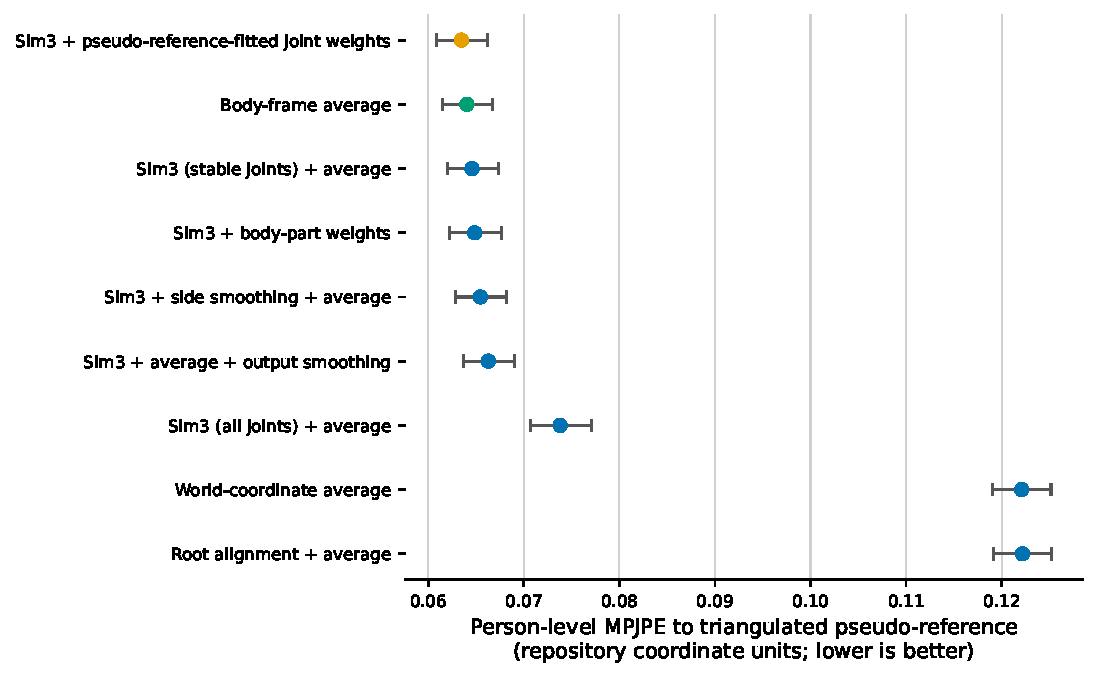
\includegraphics[width=\linewidth]{figures/deterministic_mpjpe.pdf}
\caption{Mean person-level distance to the same-video triangulated
pseudo-reference and fixed-seed 95\% bootstrap confidence interval for the
deterministic matrix. Units are repository coordinate units.}
\label{fig:deterministic}
\end{figure}

The strongest leakage-free intervals overlap. Accordingly, the deterministic
evidence supports canonicalization as the dominant operation, but does not
establish universal superiority of one eligible weighting or smoothing rule.
World-coordinate and root-aligned averages are nearly identical because the
evaluator removes root translation before scoring.

\subsection{Primary held-out learned comparison}

\begin{table*}[t]
\centering
\caption{Primary learned comparison on the held-out test set ($N=14$).
MPJPE is measured in millimeters after one sequence-level Sim3 alignment to the
same-video triangulated pseudo-reference and is reported as person-level
mean $\pm$ SD. Differences are method minus A6 with person-bootstrap 95\%
confidence intervals and Holm-adjusted paired Wilcoxon $p$-values. ROM and
peak-$\omega$ are A3-relative retention ratios; they do not use the
triangulated pseudo-reference as their denominator.}
\label{tab:learned-results}
\scriptsize
\setlength{\tabcolsep}{3pt}
\resizebox{\linewidth}{!}{%
\begin{tabular}{c l c c c c c}
\toprule
ID & Method & MPJPE (mm) & $\Delta$ vs A6 (mm) [95\% CI] &
$p_{\mathrm{Holm}}$ & A3-relative ROM & A3-relative peak-$\omega$ \\
\midrule
A0 & Face only & 77.92 $\pm$ 12.52 & +17.14 [+13.69, +21.34] & 0.0011 & 1.156 & 1.018 \\
A1 & Side only & 75.84 $\pm$ 13.93 & +15.07 [+10.23, +19.48] & 0.0018 & 1.050 & 1.654 \\
A2 & Arithmetic mean & 60.85 $\pm$ 8.98 & +0.07 [-0.50, +0.59] & 1.0000 & 1.101 & 0.917 \\
A3 & Quality mean & 61.03 $\pm$ 8.84 & +0.26 [+0.17, +0.35] & 0.0011 & 1.000 & 1.000 \\
A4 & Spatial objectives & 62.81 $\pm$ 8.86 & +2.04 [+1.71, +2.36] & 0.0011 & 0.949 & 0.828 \\
A5 & + rotation/temporal & 60.80 $\pm$ 8.96 & +0.02 [-0.38, +0.43] & 1.0000 & 0.943 & 0.644 \\
A6 & + complete-cycle ROM (mainline) & 60.78 $\pm$ 8.72 & -- & -- & 1.000 & 1.000 \\
A7 & + per-view-peak ROM & 61.31 $\pm$ 8.87 & +0.54 [+0.38, +0.69] & 0.0011 & 0.948 & 0.821 \\
A8 & + twist residual & 92.02 $\pm$ 9.59 & +31.25 [+27.78, +34.88] & 0.0011 & 1.218 & 2.187 \\
A9 & + twist-rate anchor & 94.11 $\pm$ 9.14 & +33.34 [+30.00, +36.77] & 0.0011 & 0.997 & 2.615 \\
\bottomrule
\end{tabular}
}
\end{table*}


On the held-out test set ($N=14$), A6 reaches 60.78~mm after the declared
sequence-level similarity alignment. Arithmetic averaging A2 differs from A6
by $+0.07$~mm (95\% CI $-0.50$ to $+0.59$,
$p_{\mathrm{Holm}}=1.000$), and A5 differs by $+0.02$~mm
(95\% CI $-0.38$ to $+0.43$, $p_{\mathrm{Holm}}=1.000$). These
data do not distinguish the three methods in position error. A3 is
$0.26$~mm worse (95\% CI $0.17$--$0.35$), and A7 is $0.54$~mm
worse (95\% CI $0.38$--$0.69$); both paired Holm-adjusted
$p=0.0011$. A8 and A9 degrade substantially to 92.02 and 94.11~mm.

All A2--A9 outputs are view-swap invariant to the reported precision. A6 has
A3-relative ROM and peak-$\omega$ retention of 1.000 and bone CV of 0.0190.
A7 does not reproduce the apparent all-person ROM increase on the held-out
people: its A3-relative ROM and peak-$\omega$ ratios are 0.948 and 0.821.
Thus, A6 remains the mainline because it is the complete prespecified,
auditable constrained objective, not because it wins positional accuracy.

The 137-person learned inference remains useful as a descriptive all-person
diagnostic, but it combines training, validation, and test people and is not a
generalization estimate. In particular, its apparent A7 motion-retention
advantage is not used to override the held-out result.

\subsection{Validation-only robustness diagnostics}

The fixed-corruption manifest contains 27 validation people and seven
corruption families. A6 has larger aggregate clean-to-corrupted displacement
than A4 and A5 (0.120 versus approximately 0.09 repository units); this metric
measures output movement under a challenge, not recovery toward independent
truth. Table~\ref{tab:robustness-results} details A3 and A6 by family.

\begin{table}[t]
\centering
\caption{Per-family robustness under the fixed corruption manifest (27-person
manifest subset, single seed). Each value is the person-level mean displacement
of a method's output from its own clean output, on the frames the family
corrupts (repository coordinate units); smaller means the output moves less under
that corruption.}
\label{tab:robustness-results}
\small
\begin{tabular}{l c c}
\toprule
Challenge & A3 & A6 \\
\midrule
Joint dropout & 0.0629 & 0.0873 \\
Temporal block dropout & 0.0619 & 0.0873 \\
Impulse noise & 0.0605 & 0.0605 \\
Random-walk drift & 0.0445 & 0.0445 \\
Thorax rotation bias & 0.0312 & 0.0312 \\
Frozen segment & 0.0643 & 0.0643 \\
Integer time shift & 0.0348 & 0.0348 \\
\bottomrule
\end{tabular}
\end{table}


For dropout families A6 moves more than A3, whereas shared coordinate shifts
move both outputs similarly. A temporal-offset sweep over all 137 people is
also descriptive: shifting the side map by $\pm2$ and $\pm4$ frames moves A6
by 0.046 and 0.078 repository units, essentially matching the deterministic
mean. The learned model therefore inherits rather than resolves the upstream
global-offset dependence.

\subsection{Limited Unity native-3D evaluation}

\begin{table*}[t]
\centering
\caption{Limited external evaluation against Unity native 3D (199 samples,
three sequences, one avatar/environment, Unity16 joints). All rows use one
sequence-level Sim3 before scoring. The calibrated 2D and uncalibrated direct 3D
input regimes use different evidence and supervision and must not be pooled into
a single ranking.}
\label{tab:unity-benchmark}
\small
\resizebox{\linewidth}{!}{%
\begin{tabular}{l l r r l}
\toprule
Input regime & Method & MPJPE (mm) & Angle MAE ($^\circ$) & Replication \\
\midrule
Uncalibrated direct 3D, zero-shot & World-coordinate average & 166.537 & 47.497 & -- \\
Uncalibrated direct 3D, zero-shot & A6 & 178.506 & 45.983 & -- \\
Calibrated 3D, Unity-supervised & Extrinsic gate & 153.645 & 41.090 & 2 folds $\times$ 3 seeds \\
Calibrated 2D $\rightarrow$ 3D, zero-shot & Triangulation (SAM3D 2D) & 30.259 & 15.198 & -- \\
Calibrated 2D $\rightarrow$ 3D, Unity-supervised & Learnable triangulation & 28.058 & 14.555 & 2 folds $\times$ 3 seeds \\
\bottomrule
\end{tabular}
}
\end{table*}


The independent synthetic reference changes the interpretation. Among
uncalibrated direct-3D methods, the world-coordinate average obtains
166.537~mm, whereas zero-shot A6 obtains 178.506~mm. A6 therefore provides no
external-transfer improvement in this setting. Calibrated triangulation from
SAM3D 2D evidence is much lower at 30.259~mm and 15.198$^\circ$ angle MAE.

With Unity native 3D supervision, the calibrated 3D extrinsic gate averages
153.645~mm over two folds and three seeds, a 6.74\% improvement over its
matched direct-average baseline (164.748~mm). Learnable triangulation averages
28.058~mm, 1.88\% below its matched fixed-triangulation baseline
(28.596~mm). These supervised rows answer different questions and are not
evidence that the private no-GT learner generalizes. The Unity benchmark itself
contains only one avatar/environment and a fixed camera pair, so it defines a
failure boundary rather than a population-level benchmark claim.

\subsection{Person-disjoint cohort and repeated-cycle analysis}
\label{sec:cohort-cycle-results}

\paragraph{Coverage and model diagnostics.}
The audited A6 cross-fit contains all 137 participants and 928 eligible cycles:
539 from elderly-labeled and 389 from student-labeled participants. All eight
centered primary mixed models converged without a person-permutation fallback.
Six retained person-specific random intercepts and cycle-position slopes;
axial ROM and wrist wrapping used the prespecified random-intercept fallback
because their slope covariance was singular. Maximum standardized residuals and
variance components are archived with the generated results.

\begin{table}
\centering
\caption{Out-of-fold cohort and repeated-cycle analysis. Cohort effects are elderly-minus-student mixed-model coefficients at the mid-repetition reference (normalized cycle position 0.5); angular speed, duration, and repeatability use log models. MAD effects are person-level median differences. Values are estimated kinematic descriptors, not clinical joint angles.}
\label{tab:cohort_cycle_results}
\scriptsize
\resizebox{\linewidth}{!}{%
\begin{tabular}{lcccccc}
\toprule
Outcome & Elderly median [IQR] & Student median [IQR] & Cohort effect [95\% CI] & $p_{\mathrm{Holm}}$ & MAD effect ($p_{\mathrm{Holm}}$) & Cohort$\times$cycle ($p_{\mathrm{Holm}}$) \\
\midrule
Axial rotation ROM & 0.831 [0.750, 0.971] & 0.881 [0.696, 0.979] & 0.2475 [-0.0242, 0.5192] & 0.2966 & -0.0016 (1.0000) & -0.0837 (1.0000) \\
Angular speed (P95) & 2.033 [1.714, 3.021] & 1.904 [1.675, 2.198] & 0.3006 [0.1136, 0.4876] & 0.0114 & 0.0314 (0.4459) & -0.0363 (1.0000) \\
Peak rotation phase & 0.460 [0.430, 0.904] & 0.460 [0.440, 0.900] & -0.0013 [-0.0568, 0.0542] & 1.0000 & 0.0000 (1.0000) & 0.0156 (1.0000) \\
Trunk tilt (P95) & 0.040 [0.033, 0.049] & 0.036 [0.030, 0.045] & 0.0042 [0.0002, 0.0082] & 0.2514 & -0.0002 (1.0000) & -0.0005 (1.0000) \\
Wrist wrapping (P95) & 3.021 [2.502, 3.060] & 3.027 [2.442, 3.061] & 0.0289 [-0.0626, 0.1204] & 1.0000 & -0.0073 (1.0000) & -0.0115 (1.0000) \\
Cycle duration & 2.638 [2.625, 2.650] & 2.650 [2.633, 2.667] & -0.0127 [-0.0256, 0.0002] & 0.2677 & 0.0083 (1.0000) & -0.0127 (1.0000) \\
Log dimensionless jerk & 10.178 [10.019, 10.621] & 10.097 [9.970, 10.315] & 0.4233 [0.2336, 0.6130] & 0.0001 & 0.0377 (0.0208) & -0.0167 (1.0000) \\
Whole-body repeatability & 0.016 [0.014, 0.019] & 0.016 [0.013, 0.019] & -0.0145 [-0.1055, 0.0765] & 1.0000 & -0.0003 (1.0000) & 0.0347 (1.0000) \\
\bottomrule
\end{tabular}%
}
\end{table}


\paragraph{Mid-repetition cohort contrasts.}
At normalized cycle position 0.5, the elderly coefficient for
95th-percentile angular speed is 0.3006 on the log scale (95\% CI
0.1136--0.4876, $p_{\mathrm{Holm}}=0.0114$), corresponding to a ratio of
1.351 (95\% CI 1.120--1.628). Log dimensionless angular jerk is 0.4233
higher (95\% CI 0.2336--0.6130,
$p_{\mathrm{Holm}}<0.0001$). Axial ROM, peak phase, wrist wrapping, cycle
duration, and whole-body repeatability do not show corrected cohort differences.
Trunk tilt has an uncorrected $p=0.0419$ but does not survive correction
($p_{\mathrm{Holm}}=0.2514$).

Omitting the artificial outer-fold fixed effects yields closely matched
coefficients: 0.2972 for log angular speed
($p_{\mathrm{Holm}}=0.0186$) and 0.4161 for log jerk
($p_{\mathrm{Holm}}=0.0004$). This sensitivity shows that the two primary
contrasts are not created by the outer-fold indicators.

\paragraph{Within-person cycles and repetition order.}
Only log dimensionless jerk shows a corrected cohort difference in
within-person dispersion. The elderly-minus-student difference in person-level
MAD is 0.0377 (bootstrap 95\% CI 0.0135--0.0735,
$p_{\mathrm{Holm}}=0.0208$). None of the other seven MAD contrasts survives
correction. All eight cohort-by-cycle-position interactions have
$p_{\mathrm{Holm}}=1.000$. The data therefore provide no evidence for a
different monotonic first-to-last repetition trend between cohorts.

\begin{figure}
\centering
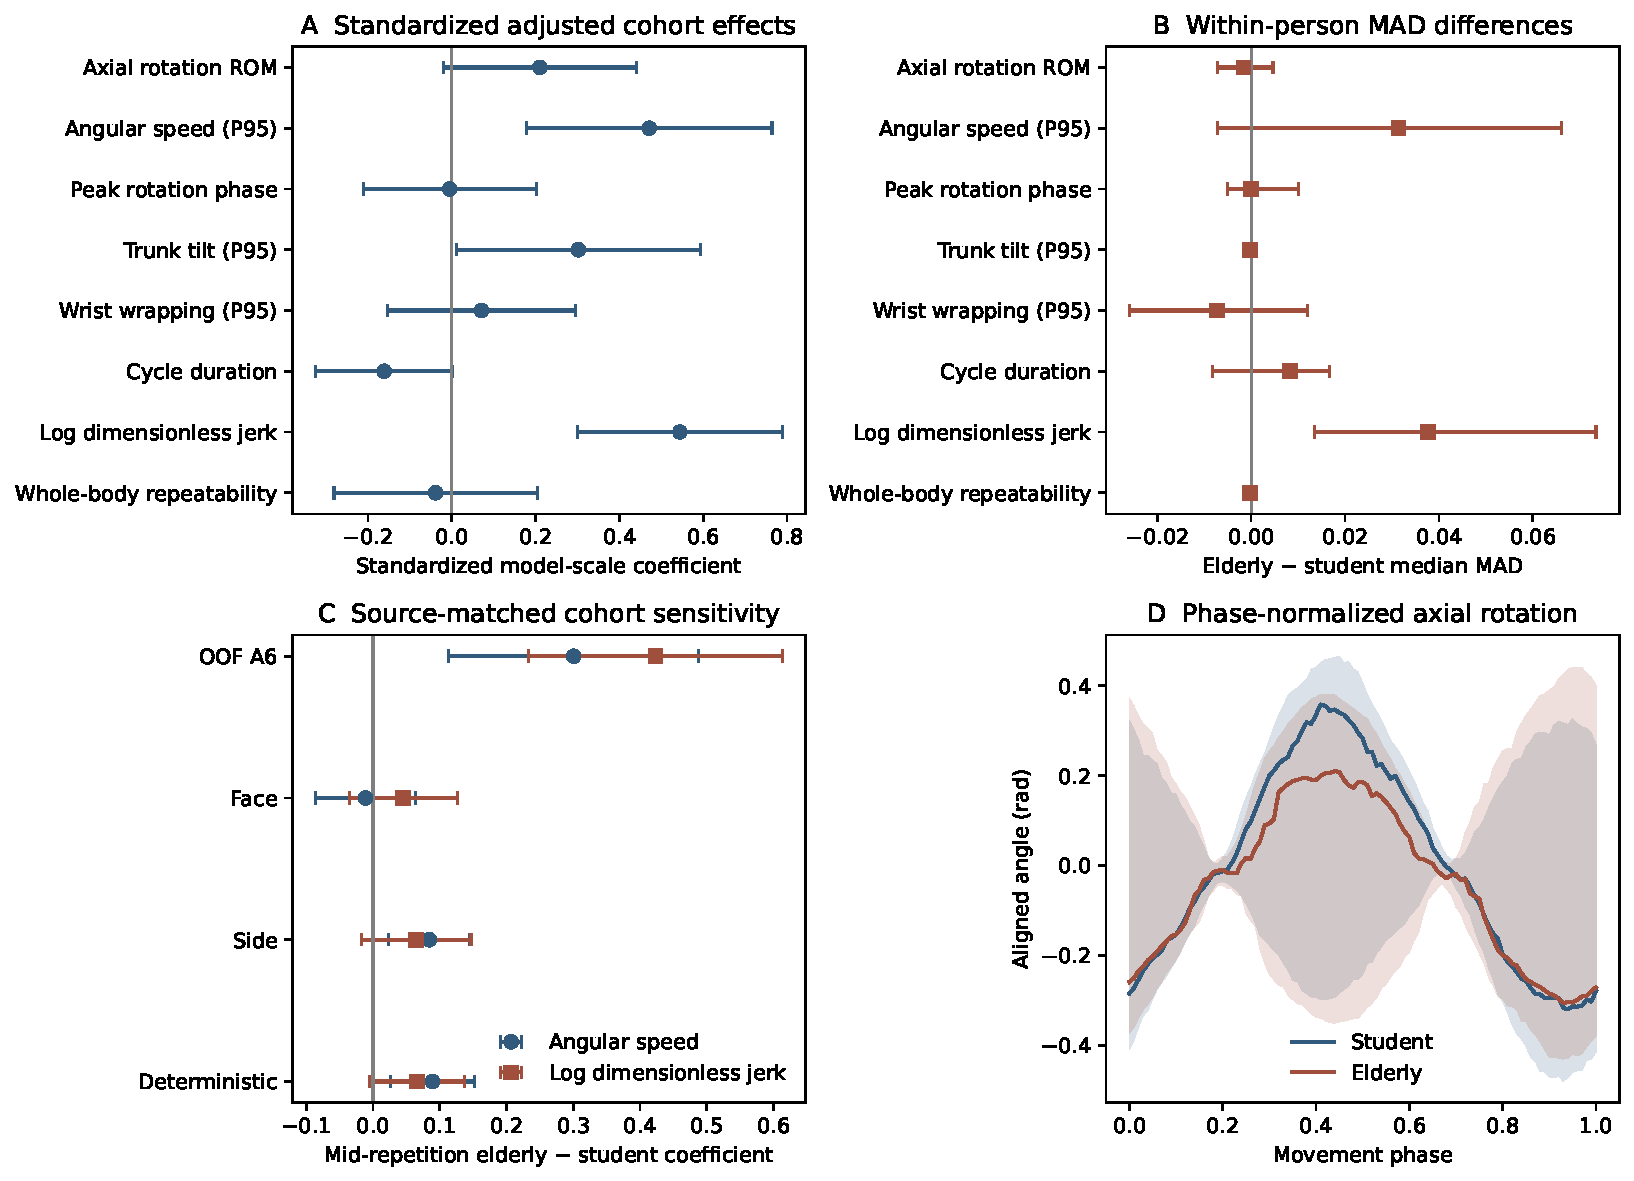
\includegraphics[width=\linewidth]{figures/cohort_cycle_analysis.pdf}
\caption{Person-disjoint cohort analysis. (A) Standardized mid-repetition
mixed-model cohort effects. (B) Person-level within-person MAD differences.
(C) Source-matched centered mixed-model sensitivity for angular speed and log
dimensionless jerk. Error bars are 95\% confidence intervals. (D)
Person-median phase-normalized axial rotation with interquartile bands; no
axial-angle cluster survives correction across descriptor families.}
\label{fig:cohort-cycle-analysis}
\end{figure}

\paragraph{Phase-localized comparisons.}
No axial-angle or angular-speed cluster is significant after across-descriptor
Holm correction. Trunk-tilt clusters remain at phases 0.19--0.36 and
0.73--0.87 (both adjusted $p=0.0040$) and 0.91--1.00
($p=0.0130$). Wrist wrapping differs over phase 0.30--0.57
($p=0.0237$). These secondary, model-derived localizations are
hypothesis-generating and not anatomical validation.

\begin{table*}[t]
\centering
\caption{Pose-source sensitivity using the same centered cycle-level mixed model
as the primary analysis. Cells report the mid-repetition
elderly-minus-student coefficient [95\% CI] with
$p_{\mathrm{Holm}}$ corrected across eight outcomes within each source.}
\label{tab:cohort-cycle-sensitivity}
\scriptsize
\resizebox{\linewidth}{!}{%
\begin{tabular}{l c c c c}
\toprule
Outcome & OOF A6 & Face only & Side only & Deterministic \\
\midrule
Angular speed (P95) & 0.3006 [0.1136, 0.4876] (0.0114) & -0.0111 [-0.0861, 0.0639] (1.0000) & 0.0843 [0.0233, 0.1452] (0.0337) & 0.0891 [0.0264, 0.1519] (0.0323) \\
Log dimensionless jerk & 0.4233 [0.2336, 0.6130] (0.0001) & 0.0452 [-0.0357, 0.1261] (1.0000) & 0.0646 [-0.0177, 0.1468] (0.2475) & 0.0657 [-0.0056, 0.1369] (0.2324) \\
\bottomrule
\end{tabular}%
}
\end{table*}


\paragraph{Pose-source sensitivity.}
Applying the same centered cycle-level model to each pose source materially
changes the magnitude. For log angular speed, the cohort coefficient is
0.3006 for OOF A6, $-0.0111$ for face, 0.0843 for side, and 0.0891 for
deterministic fusion; only A6, side, and deterministic fusion survive their
within-source Holm families. For log jerk, A6 is 0.4233, whereas face, side,
and deterministic estimates are 0.0452, 0.0646, and 0.0657 and none of the
latter is corrected-significant. The A6 application signals are therefore
pose-source-sensitive and may reflect learned representation effects as well as
movement differences.

As a separate participant-balanced estimand, person-median permutations do not
show corrected A6 differences for angular speed
($p_{\mathrm{Holm}}=0.8783$) or jerk
($p_{\mathrm{Holm}}=0.5159$). This estimand difference further limits the
cohort analysis to an exploratory application demonstration.

\section{Discussion}
\label{sec:discussion}

\subsection{Canonicalization explains most private-data improvement}

The strongest reproducible private-data result is deterministic. Removing
inter-view translation, orientation, and scale mismatch nearly halves
pseudo-reference distance relative to world-coordinate averaging. Several
leakage-free canonical methods then lie within a narrow range with overlapping
intervals. This supports coordinate normalization as the dominant operation,
not a claim that a particular learned weighting is universally superior.

The 14-person held-out test reinforces that boundary. A6, A5, and arithmetic
averaging are statistically indistinguishable in MPJPE. A6 should therefore be
read as an auditable constrained extension: it makes the self-supervised
recovery, skeletal, temporal, rotation, complete-cycle, and swap-invariance
assumptions explicit while bounding departure from A3. It has no demonstrated
positional advantage.

\subsection{Rotation diagnostics require the correct denominator}

Smoothness and coordinate error do not uniquely characterize rotation. The
method explicitly represents pelvis--thorax rotation and complete-cycle range
to reveal attenuation or overshoot. However, the reported ROM and
peak-angular-velocity retention ratios are relative to A3, not to triangulated
motion. They show how far a learned variant departs from its deterministic
base. On the held-out test, A7 retains less A3 range and peak speed than A6;
the descriptive all-person A7 increase does not reproduce. The freer A8/A9
residuals markedly worsen MPJPE and over-amplify peak angular velocity. These
findings support retaining conservative A6 constraints, but not calling A3 or
A6 biomechanically accurate.

\subsection{Unity exposes an external-transfer boundary}

Unity native 3D is independent of the private triangulated pseudo-reference,
although it is synthetic and limited to one avatar/environment. A6 performs
worse than direct world-coordinate averaging under zero-shot direct-3D input.
The result rejects an external positional-transfer claim for the current
learner. It also shows that a normalization that agrees with a private
same-video pseudo-reference need not preserve Unity coordinates after the
declared evaluation alignment.

Calibrated 2D triangulation is far more accurate in Unity than any direct
monocular-3D fusion row. This is not a contradiction: projection geometry and
2D evidence contain information unavailable after two monocular 3D predictions
have already been produced. The modest gains from Unity-supervised extrinsic
gating and learnable triangulation further show what becomes possible once
camera geometry and native 3D supervision are authorized. These different
regimes should guide deployment choices rather than be pooled into one ranking.

\subsection{The cohort application is representation-sensitive}

Centering cycle position makes the primary cohort coefficient representative of
the observed repetitions rather than conditional on the first detected cycle.
Angular speed and log jerk remain corrected-significant with and without
outer-fold fixed effects, while no cohort-by-repetition interaction survives.
Log jerk also has greater within-person MAD in the elderly-labeled cohort.

The source-matched analysis is a stronger qualification than the original
person-median comparison because it uses the same cycle-level mixed-model
estimand for every pose stream. A6 produces substantially larger cohort
coefficients than face, side, or deterministic fusion, especially for log
jerk. The result may combine movement execution, cohort composition,
pose-estimation error, and A6 representation effects. Without individual ages,
health, training history, anthropometry, or independent kinematics, these
mechanisms cannot be separated. The appropriate contribution is an auditable
hypothesis-generation workflow, not an ageing or clinical conclusion.

\subsection{Relation to calibrated motion analysis}

The proposed method addresses a downstream regime in which two complete
monocular 3D streams already exist and camera parameters are unavailable.
Learnable triangulation and camera-aware fusion instead use images or 2D
evidence to recover geometrically grounded 3D pose
\citep{Iskakov2019Learnable,Qiu2019CrossView,Remelli2020Lightweight}. Systems
such as OpenCap additionally use calibrated capture, Mocap-trained modeling,
musculoskeletal constraints, and laboratory validation
\citep{Uhlrich2023OpenCap}. A fused face-reference sequence from the present
pipeline is therefore suitable for comparative sequence descriptors and
downstream modeling, but not for validated joint angles, forces, or moments.

Future validation should add diverse public multi-view data or synchronized
independent capture. Human3.6M, MPI-INF-3DHP, and TotalCapture offer increasing
variation or independent modalities
\citep{Ionescu2014Human36M,Mehta2017MPIINF3DHP,Trumble2017TotalCapture}.
Applying the same post-estimation protocol would test whether the negative
Unity transfer result generalizes across people, cameras, and movements.

\section{Limitations}
\label{sec:limitations}

\paragraph{Private pseudo-reference.}
The private triangulated evaluator uses 2D evidence from the same videos as the
monocular 3D inputs. Its errors can be correlated with candidate errors, and
sequence-level Sim3 plus hip centering removes some failure modes before
scoring. Private MPJPE is agreement with one upstream construction, not
absolute 3D accuracy.

\paragraph{Small single-seed held-out study.}
The primary learned test contains only 14 people and one training seed. Paired
tests control person reuse across methods but do not estimate optimization
variance or broad population uncertainty. The 137-person learned values include
training and validation participants and are descriptive only.

\paragraph{Limited synthetic external validation.}
Unity provides native 3D independent of the private pseudo-reference, but only
199 samples, three sequences, one avatar/environment, and one fixed camera
pair. It cannot establish population generality. Its negative A6 result and the
advantage of calibrated triangulation should be replicated on diverse real
multi-view benchmarks.

\paragraph{Observational cohort labels and unmeasured confounding.}
Elderly and student are dataset group labels, not randomized exposures.
Individual age, sex, health, training history, body size, and other covariates
are unavailable. Person-disjoint inference prevents direct train/test leakage
but does not make the comparison causal. The reported coefficients cannot be interpreted as ageing effects,
normative values, impairment markers, or clinical evidence.

\paragraph{Pose-source and estimand sensitivity.}
The A6 speed and jerk coefficients are much larger than the same centered
mixed-model coefficients from face, side, or deterministic features.
Person-median A6 comparisons are also not corrected-significant. This
instability limits the application to hypothesis generation until independent
kinematics and repeated cross-fit seeds are available.

\paragraph{Dependence on upstream errors.}
Both views originate from one monocular estimator and skeletal model.
Canonicalization cannot correct shared joint-definition, anthropometric, or
hallucination errors. High-consensus identity may reinforce common bias, and
synthetic corruptions cannot span the full real error distribution.

\paragraph{Alignment, views, and movement specificity.}
The loader honors one global side-to-face offset and does not model drift,
dropped frames, rolling shutter, or nonlinear local misalignment. Only one
face/side pair and one gymnastics movement family are studied. The architecture
is symmetric to view order but does not support a variable number of cameras.

\paragraph{Coordinate and anatomical interpretation.}
The output is restored to an uncalibrated face reference. Pelvis and thorax
frames depend directly on estimated hips and shoulders, and A3-relative
retention is not a comparison to physical motion. The method does not estimate
validated clinical joint angles, forces, or moments.

\paragraph{Model and governance choices.}
Loss weights, residual bounds, and corruption probabilities are manually
specified. Ethics approval or exemption, participant consent wording,
institutional postal address, and release conditions for code and derived data
remain author-governance items that must be verified before submission.

\section{Conclusion}
\label{sec:conclusion}

This work formulates two-view 3D pose fusion after monocular estimation. A6
combines pelvis-centered canonicalization, a transparent quality-weighted base,
a view-swap-invariant bounded temporal residual, and self-supervised recovery,
skeletal, temporal, rotation, and complete-cycle constraints without reading
triangulated targets during training or selection.

The evidence supports a narrower conclusion than positional superiority.
Canonicalization accounts for most improvement against the private same-video
pseudo-reference. On 14 held-out people, A6 is statistically
indistinguishable from arithmetic averaging and A5. It remains the method
mainline as the complete auditable constrained objective. On limited Unity
native 3D, A6 does not improve zero-shot direct-3D transfer, while calibrated
2D triangulation is substantially more accurate. This negative result marks the
boundary of uncalibrated post-estimation fusion rather than weakening the
importance of geometry.

OOF A6 features support a person-disjoint application over 928 cycles, but the
elderly--student speed and jerk coefficients are materially pose-source- and
estimand-sensitive, and no cohort-specific repetition trend survives
correction. The cohort analysis is therefore exploratory and observational.
The method is best interpreted as an auditable motion-representation layer;
diverse independent capture, repeated seeds, measured participant covariates,
and completed governance documentation are required before absolute,
biomechanical, causal, or clinical claims.

\section*{Declaration of competing interest}
The author declares that there are no known competing financial interests or
personal relationships that could have appeared to influence the work reported
in this paper.

\section*{Funding}
This research did not receive any specific grant from funding agencies in the
public, commercial, or not-for-profit sectors.

\section*{Ethics and consent}
\submissionpending{Insert the confirmed institutional ethics approval or
exemption identifier and participant consent statement before submission. No
ethics status is inferred from the repository.}

\section*{Data availability}
The raw videos contain identifiable participant information and are not
publicly available. At the time of this draft, the code and derived anonymized
keypoint data have not been deposited in a public repository. Their release and
the conditions for controlled access will be determined after institutional
ethics, participant-consent, and privacy review. All numerical results reported
in the deterministic, held-out learned, Unity, and cohort tables are generated
or copied from archived CSV/JSON artifacts by the manuscript asset script.

\section*{Declaration of generative AI and AI-assisted technologies in the
writing process}
During preparation of this work, the author used OpenAI Codex to support
manuscript organization, language editing, LaTeX preparation, and code-assisted
consistency checks. The author reviewed and edited the resulting material and
takes full responsibility for the content of the publication.

\section*{Acknowledgments}
No additional acknowledgments are declared in this draft.


\printcredits

\bibliographystyle{cas-model2-names}
\bibliography{references}

\end{document}
